\documentclass[a4paper]{jarticle}
\usepackage{comment}
\usepackage[top=20truemm,bottom=20truemm,left=20truemm,right=20truemm]{geometry}
\usepackage[dvipdfmx]{graphicx}
\usepackage{here}
\usepackage[utf8]{inputenc}
\title{ヒューマンコンピュータインタラクション\\レポート}
\author{学生番号 氏名}
\begin{document}
\maketitle
\section{課題}
身の回りにある製品(ハードウェアでもソフトウェアでも構いません)について、使いにくいと感じた点を文書にまとめてください。適宜、具体的な写真を文書に取り込むと言ったことなどをしてください。
\section{解答}
今回はkaoriyaさんがhttp://www.kaoriya.net/software/vim/で配布されているwindows向けのvimの使いにくい点についてまとめた。このソフトウェアはwindowsのコマンドプロンプト上でlinuxなどで使われるvimとほぼ同じ操作でテキストを編集できるエディタで、プログラミングやレポートの作成などで使用している。このソフトウェアを使用中インサートモードに入っているとき、マウスでコマンドプロンプトの中をクリックすると、カーソルがクリックした場所に移動してしまう。ノートパソコンでこのソフトを使うとき、意図せずにタッチパネルにふれてカーソルが移動してしまうことがある。タッチパネルを無効にすればこの現象がおきないが、使用するたびにタッチパネルを無効にし、vimを終了するたびにタッチパネルを有効にするのは不便である。
%インサートモードで文字を打ち込んでいる時
\begin{figure}[H]
	\begin{center}
		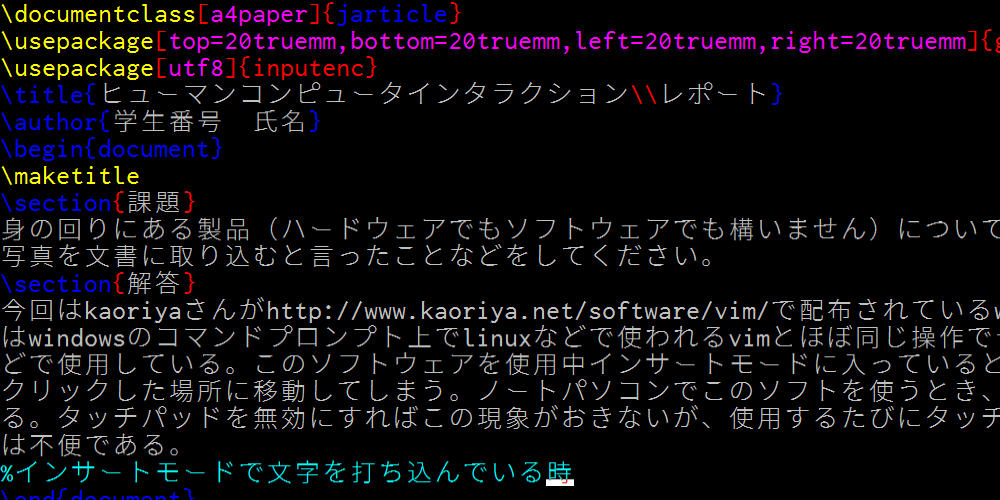
\includegraphics[width=15cm]{screenshot1edited.png}
		\caption{インサートモードで文字を打ち込んでいる時の画面}
		\label{screenshot1edited}
	\end{center}
\end{figure}
\begin{figure}[H]
	\begin{center}
		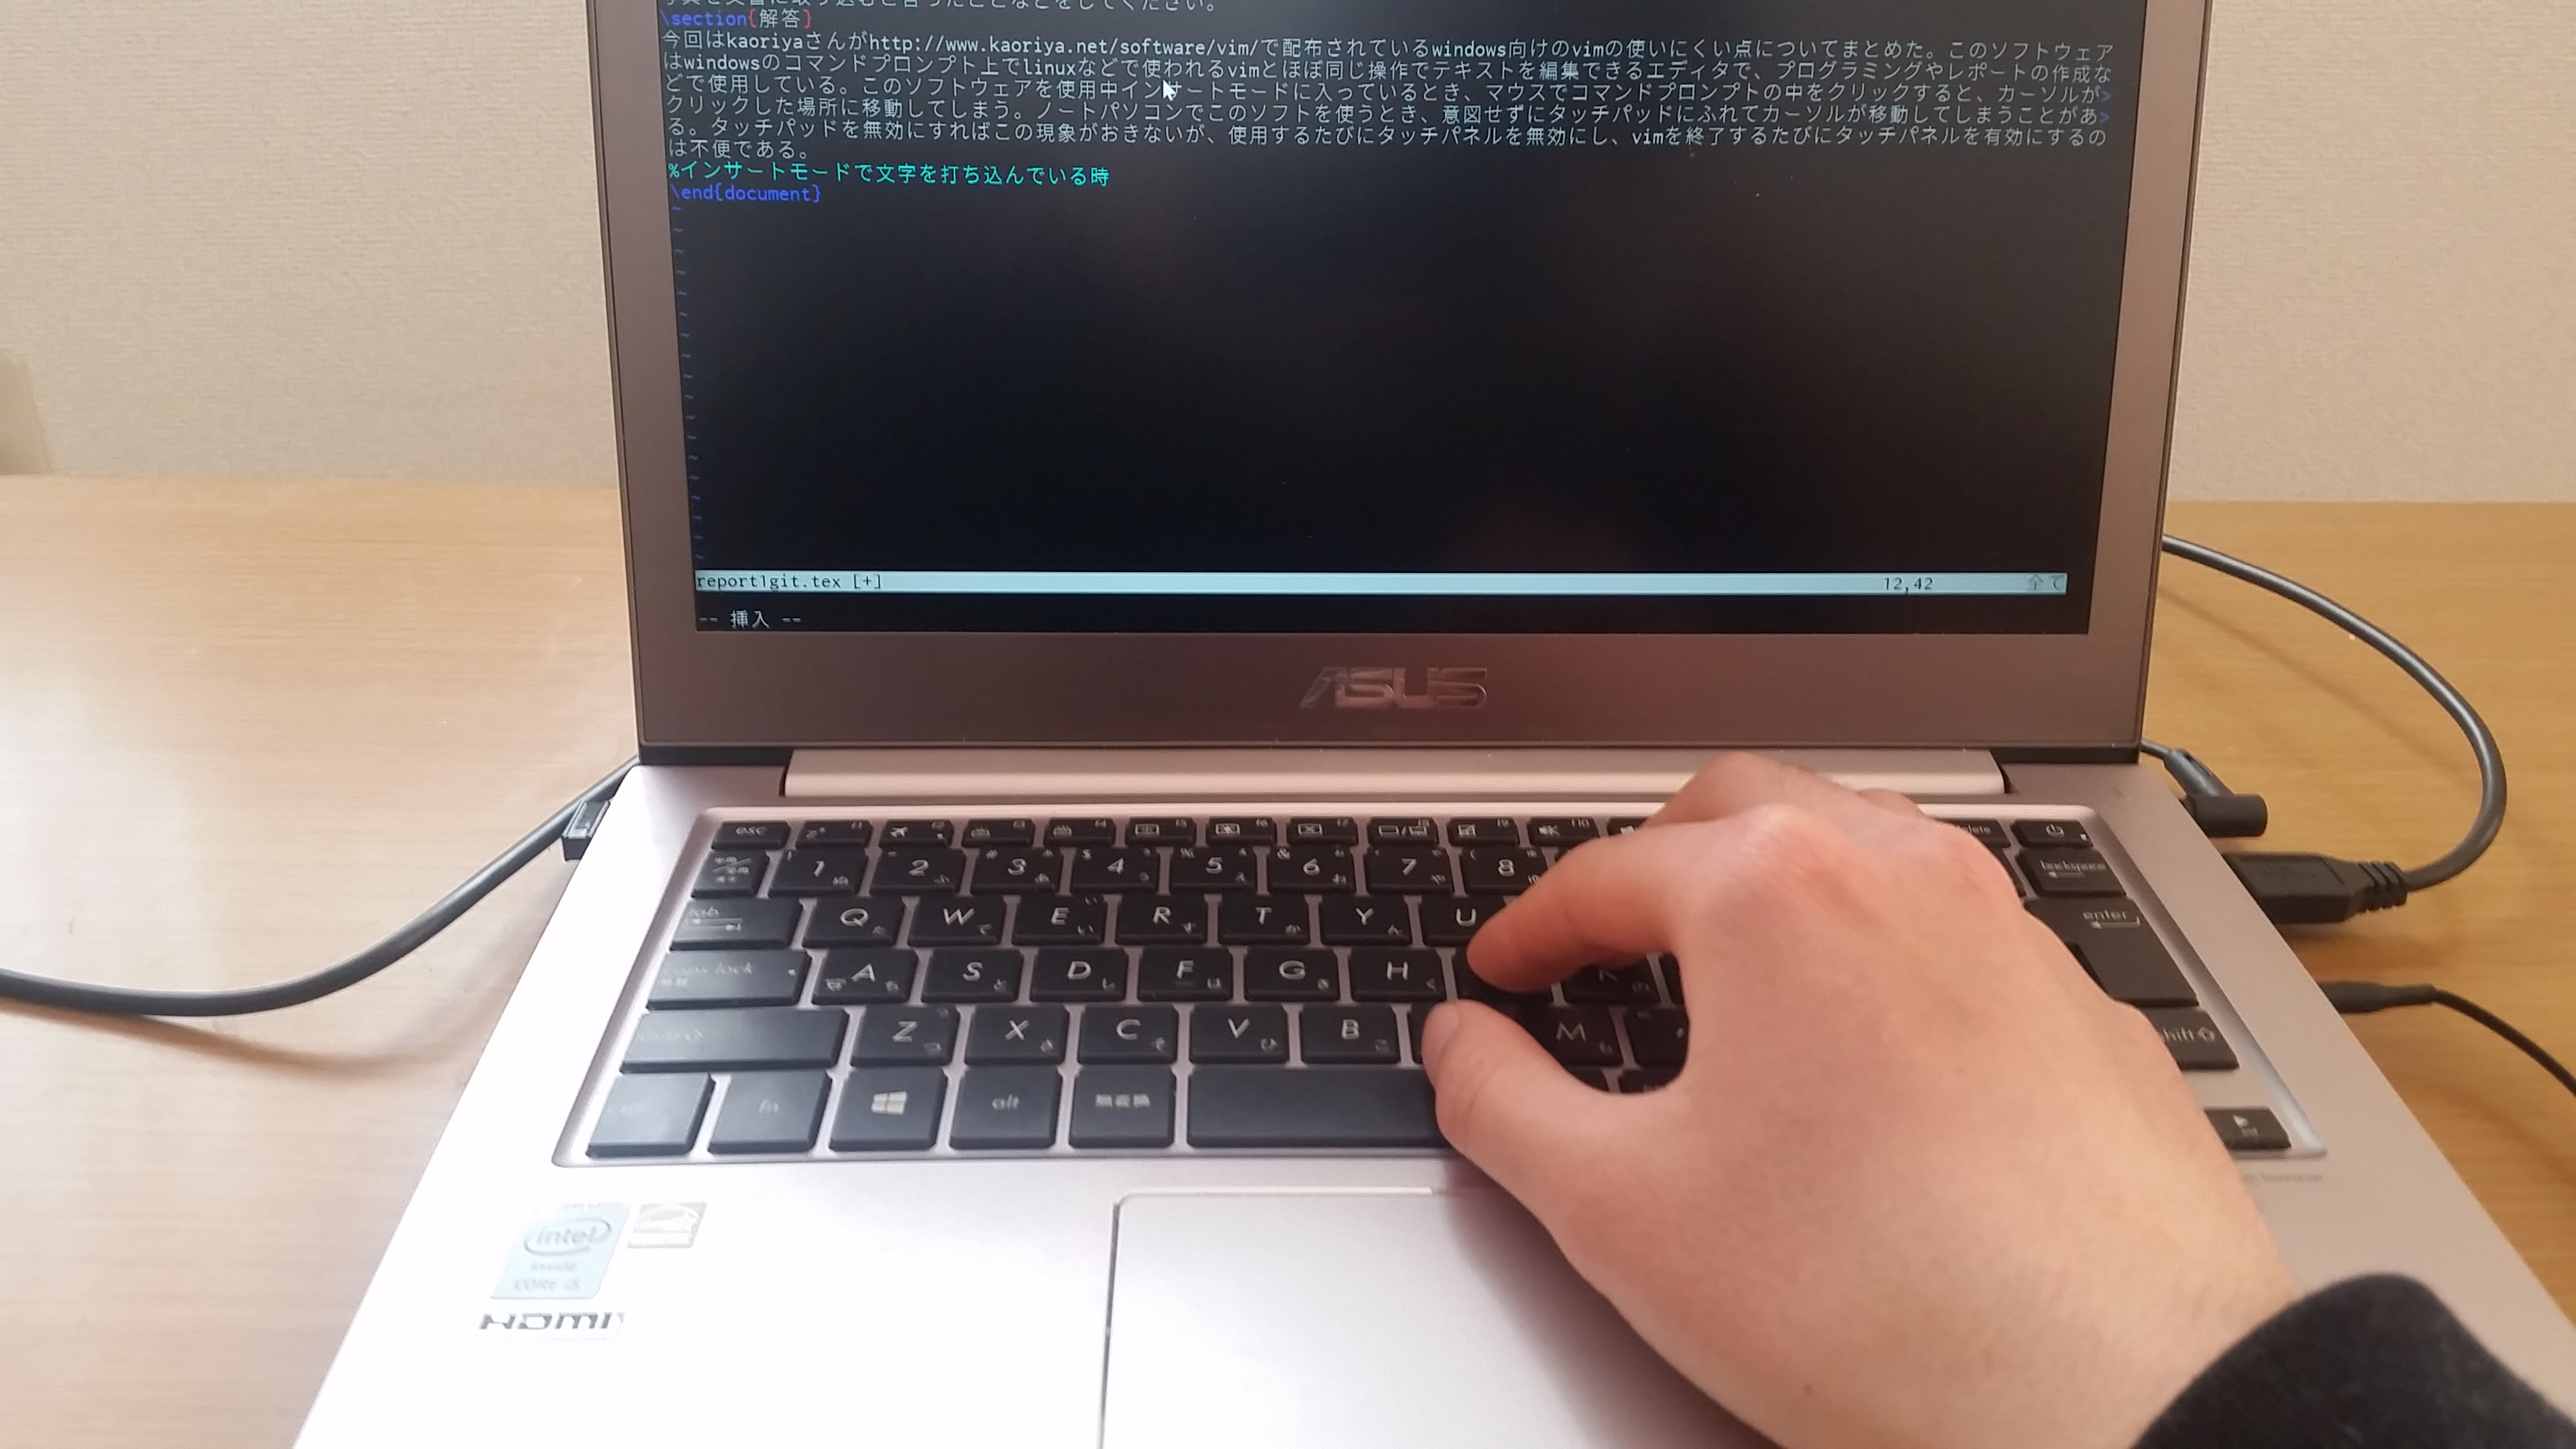
\includegraphics[width=15cm]{picture1.jpg}
		\caption{インサートモードで文字を打ち込んでいる時の様子}
		\label{picture1}
	\end{center}
\end{figure}
\begin{comment}
\begin{figure}[H]
	\begin{center}
		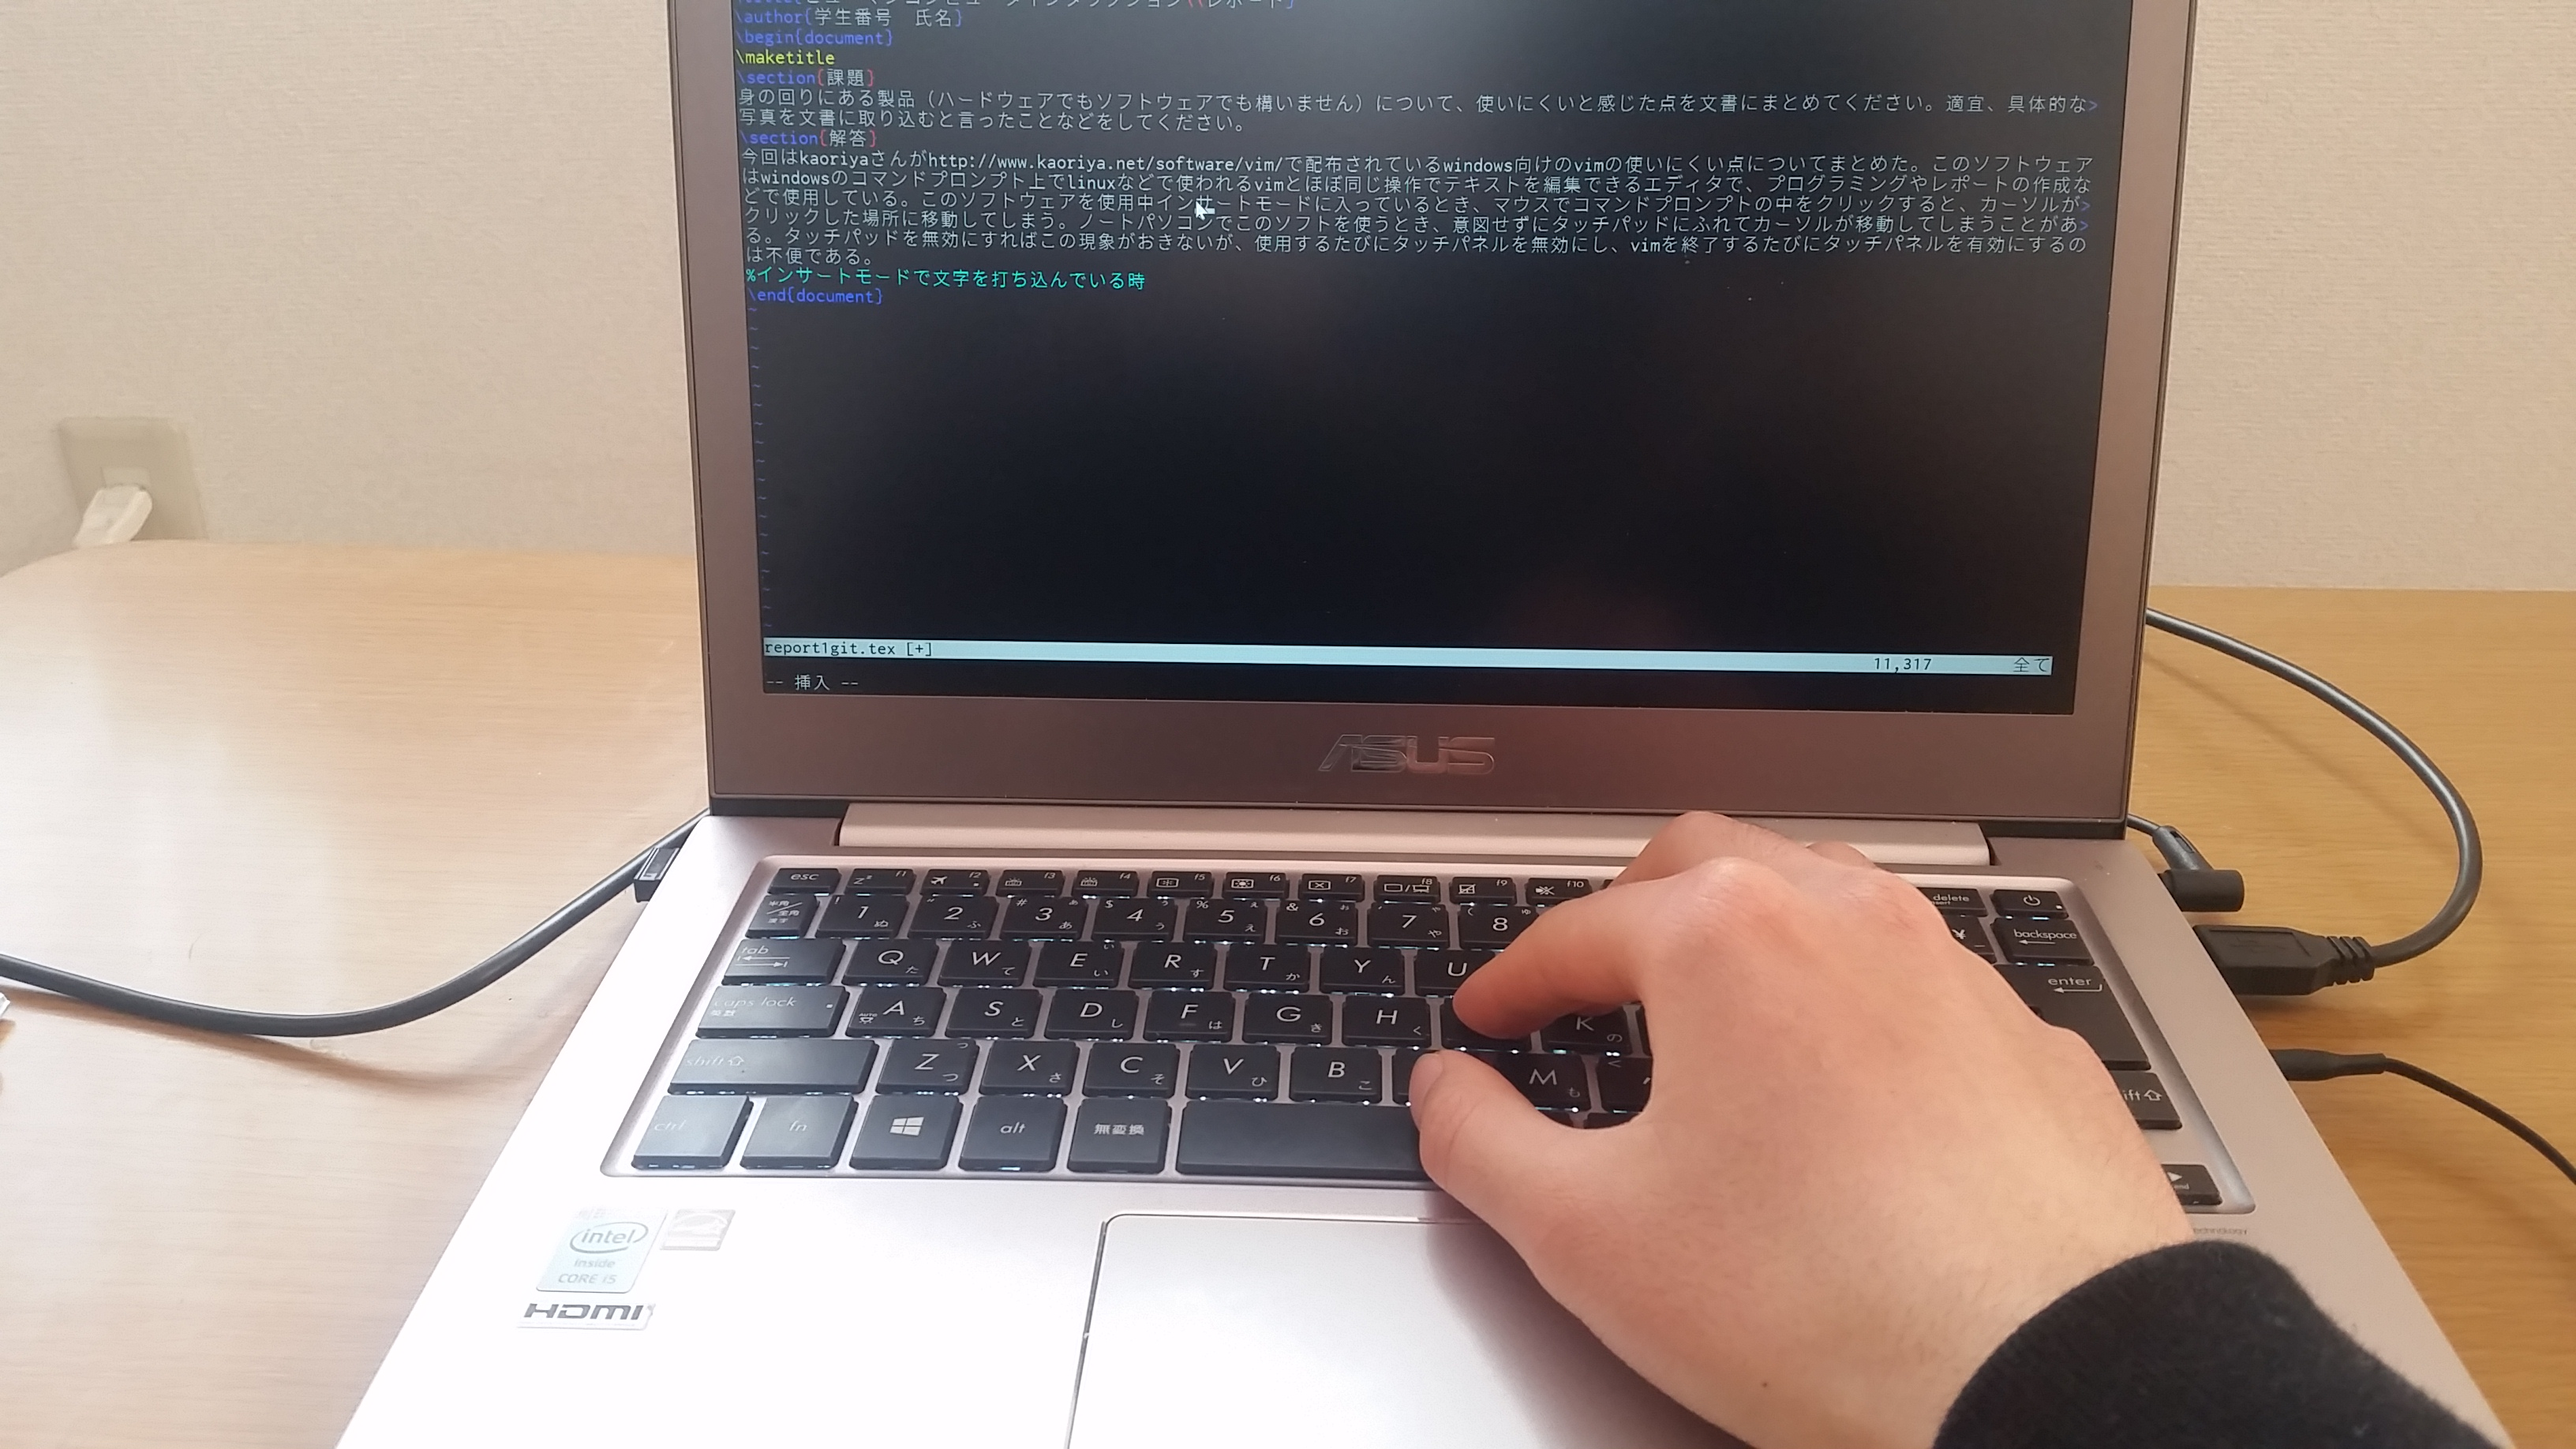
\includegraphics[width=15cm]{picture2.jpg}
		\caption{タッチパネルに触れカーソルが意図せずに移動してしまったときの様子}
		\label{picture2}
	\end{center}
\end{figure}
\end{comment}
\begin{figure}[H]
	\begin{center}
		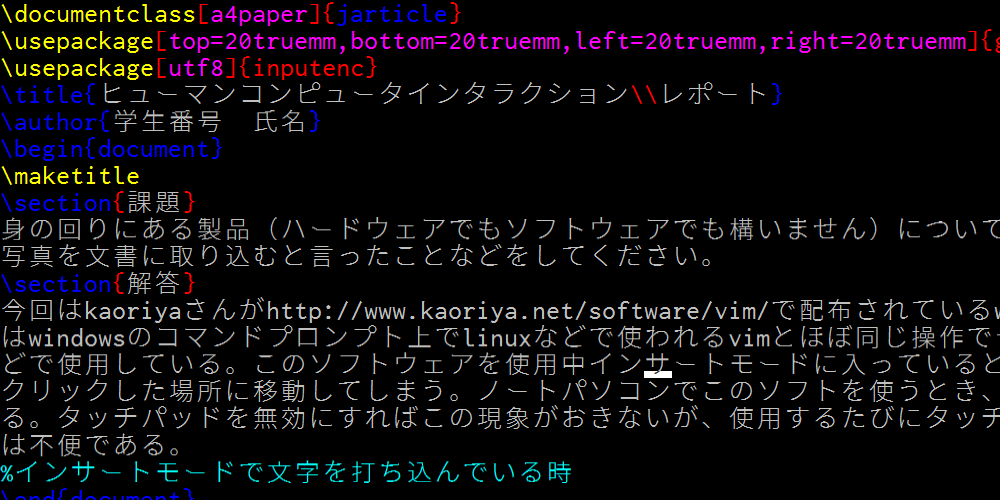
\includegraphics[width=15cm]{screenshot2edited.png}
		\caption{タッチパネルに触れカーソルが意図せずに移動してしまったときの画面}
		\label{screenshot2edited}
	\end{center}
\end{figure}
\begin{figure}[H]
	\begin{center}
		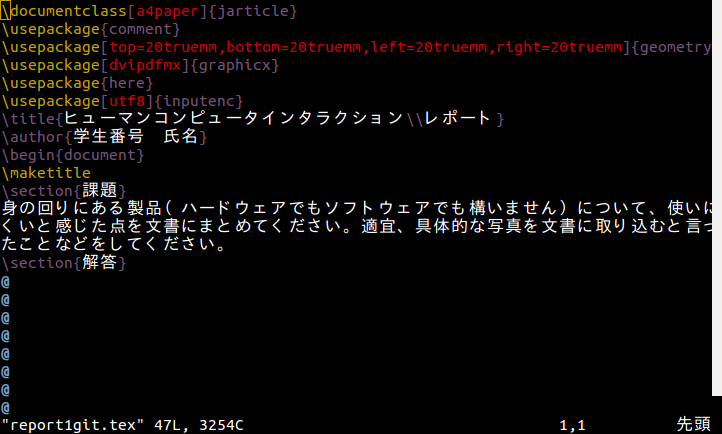
\includegraphics[width=15cm]{linuxscreenshot.png}
		\caption{AV実習室のlinuxのvim}
		\label{linuxscreenshot}
	\end{center}
\end{figure}
図\ref{screenshot1edited}のようにインサートモードで文字を打ち込んでいる時に、図\ref{picture1}のように誤って手首でタッチパネルに触れてしまうことがある。そうすると、図\ref{screenshot2edited}のようにマウスカーソルがあった場所にカーソルが意図せずに移動してしまう。私はVirtual Boxでlinuxの仮想環境を使用しているが、その中に入っているvimではターミナルの画面上をクリックしてもカーソルが移動することはなかった。図\ref{linuxscreenshot}のように、大学のAV実習室のlinuxのvimの場合も同様に画面上をクリックしてカーソルが移動することはなかった。
\section{考察}
調べた結果同じvimでもvimもどきのようなものが多くの人たちによって作られていて、それぞれに特徴があることがわかった。ただ、vimはキーボードのみで操作するものだと思うので、マウスに反応する必要はないと思った。
\end{document}
